% ==============================================================
% --- Git
% ==============================================================
\section{Basic Tasks}\hypertarget{sec2}{}

\begin{frame}[fragile]
\emptyframetitle
  In this section
  \begin{itemize}
    \item \hyperlink{sec2.1}{Setting Up Git}
    \item \hyperlink{sec2.2}{Creating A Git Repository}
    \item \hyperlink{sec2.3}{Tracking Changes}
    \item \hyperlink{sec2.4}{Exploring History}
  \end{itemize}
\end{frame}

\subsection{Setting Up Git}\hypertarget{sec2.1}{}

\begin{frame}[fragile]
\emptyframetitle

  Git comes in many different forms. We use \textbf{Git on the command line}.

  \begin{itemize}
  \item It's the only place you can run \textbf{all} Git commands.
  \item If you know the command line version, you can figure out how to run the GUI version.
  \item Everyone has the same command line tools.
  \end{itemize}

  \vspace*{0.15cm}
  On Linux 
  \begin{itemize}
    \item[] \texttt{\$ sudo dnf install git-all} (Fedora) 
    \item[] \texttt{\$ sudo apt install git-all} (Debian)
  \end{itemize}
  \vspace*{0.15cm}

  On Mac 
  \begin{itemize}
    \item[] \texttt{\$ brew install git} (Homebrew) 
    \item[] \texttt{\$ port install git} (Macports)
    \item[] part of XCode IDE
  \end{itemize}
  \vspace*{0.15cm}

  On Windows 
  \begin{itemize}
    \item[] Git for Windows: \url{https://git-scm.com/download/win} 
    \item[] GitHub Desktop: \url{https://desktop.github.com}
    \item[] Git Chocolatey: \url{https://chocolatey.org/packages/git}
  \end{itemize}

\end{frame}

\begin{frame}[fragile]
\emptyframetitle
  When we use Git for the first time, we need to configure a few things.\\[0.25cm]

  Here are a few examples of configurations we will set as we get started with Git:
  \begin{itemize}
    \item your name and email address
    \item and that we want to use these settings globally (i.e. for every project)
  \end{itemize}
  On a command line, Git commands are written as \texttt{\textbf{git verb options}}, where \texttt{\textbf{verb}} is what we actually want to do and \texttt{\textbf{options}} is additional optional information which may be needed for the verb.\\[0.25cm]

  So here is how Dracula sets up his new laptop:

  \begin{lstlisting}[language=bash]
    $ git config --global user.name "Vlad Dracula"
    $ git config --global user.email "vlad@tran.sylvan.ia"
  \end{lstlisting}

\end{frame}

\begin{frame}[fragile]
\emptyframetitle

  Quite helpful and important are the commands to look up the manual\\[0.25cm] 

  For a general overview of a range of Git commands
  \begin{lstlisting}[language=bash]
    $ git --help
  \end{lstlisting}

  For a overview of specific Git command (here command = \texttt{verb})
  \begin{lstlisting}[language=bash]
    $ git verb -h
  \end{lstlisting}

  For an in-depth manual of specific Git command
  \begin{lstlisting}[language=bash]
    $ git verb --help
  \end{lstlisting}

  \vspace*{0.5cm}
  For more information please check the \textbf{Git online documentation} at
  \url{https://git-scm.com/docs}

\end{frame}

\subsection{Creating A Git Repository}\hypertarget{sec2.2}{}


\begin{frame}[fragile]
\emptyframetitle

  Create a directory in your current working directory
  \begin{lstlisting}[language=bash]
    $ mkdir git_exercise
  \end{lstlisting}

  Change to the new directory
  \begin{lstlisting}[language=bash]
    $ cd git_exercise
  \end{lstlisting}

  Create the Git repository
  \begin{lstlisting}[language=bash]
    $ git init
  \end{lstlisting}

  \begin{block}{Note}
An invisible file \texttt{.git} is created that stores all the history and dependencies of the repository.
  \end{block}

\end{frame}

\subsection{Tracking Changes}\hypertarget{sec2.3}{}

\begin{frame}[fragile]
\emptyframetitle

  Think of Git as taking snapshots of your project in a two-step process:
  \begin{itemize}
    \item \texttt{\textbf{git add}} specifies \textbf{what} will go into a snapshot
    \item \texttt{\textbf{git commit}} \textbf{takes the actual snapshot} and records it permanently
  \end{itemize}

  \begin{figure}[h]
    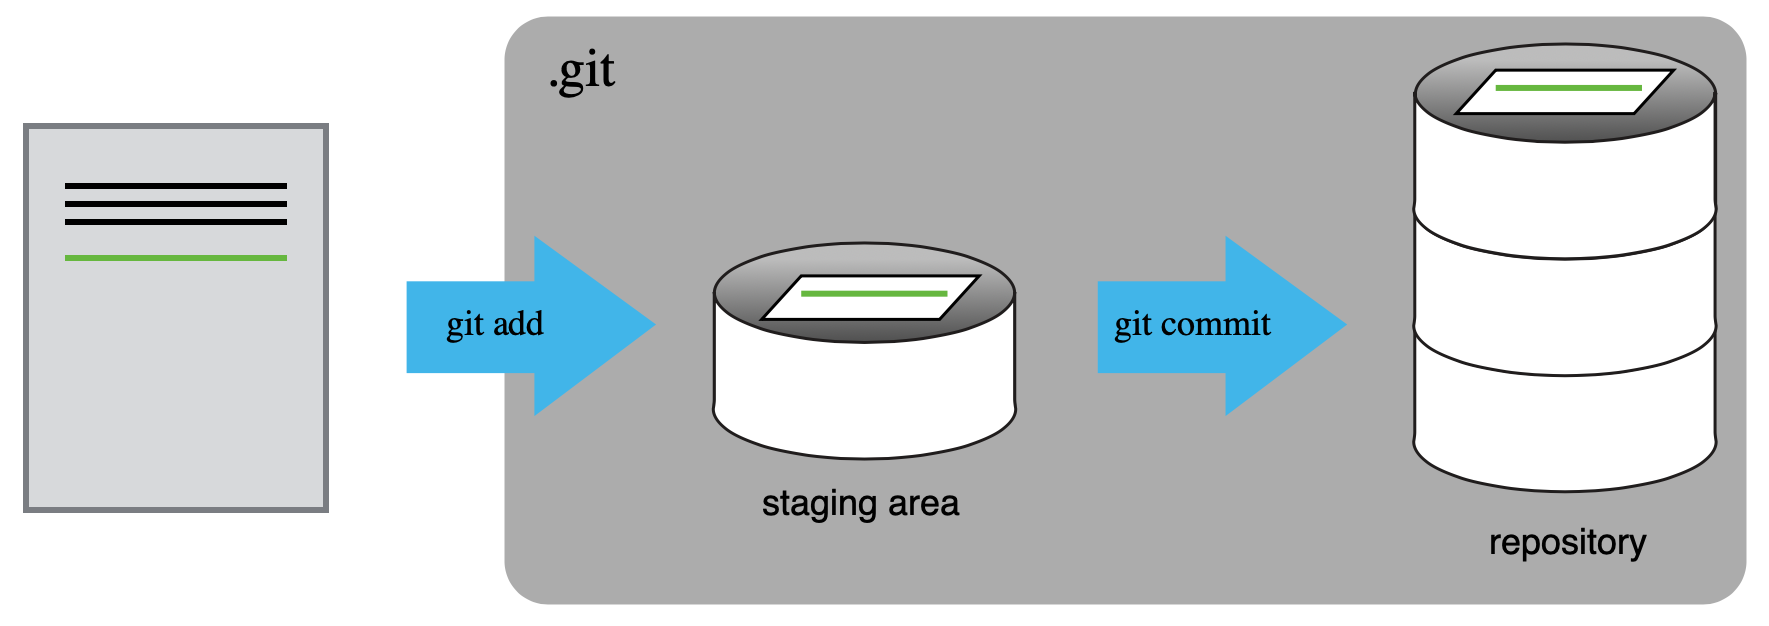
\includegraphics[width=1.0\textwidth]{sec2/git-staging-area.png}
  \end{figure}

\end{frame}

\begin{frame}[fragile]
\emptyframetitle

  It is of course possible to add multiple files (or changes thereof) before committing these, i.e. taking the snapshot.

  \begin{figure}[h]
    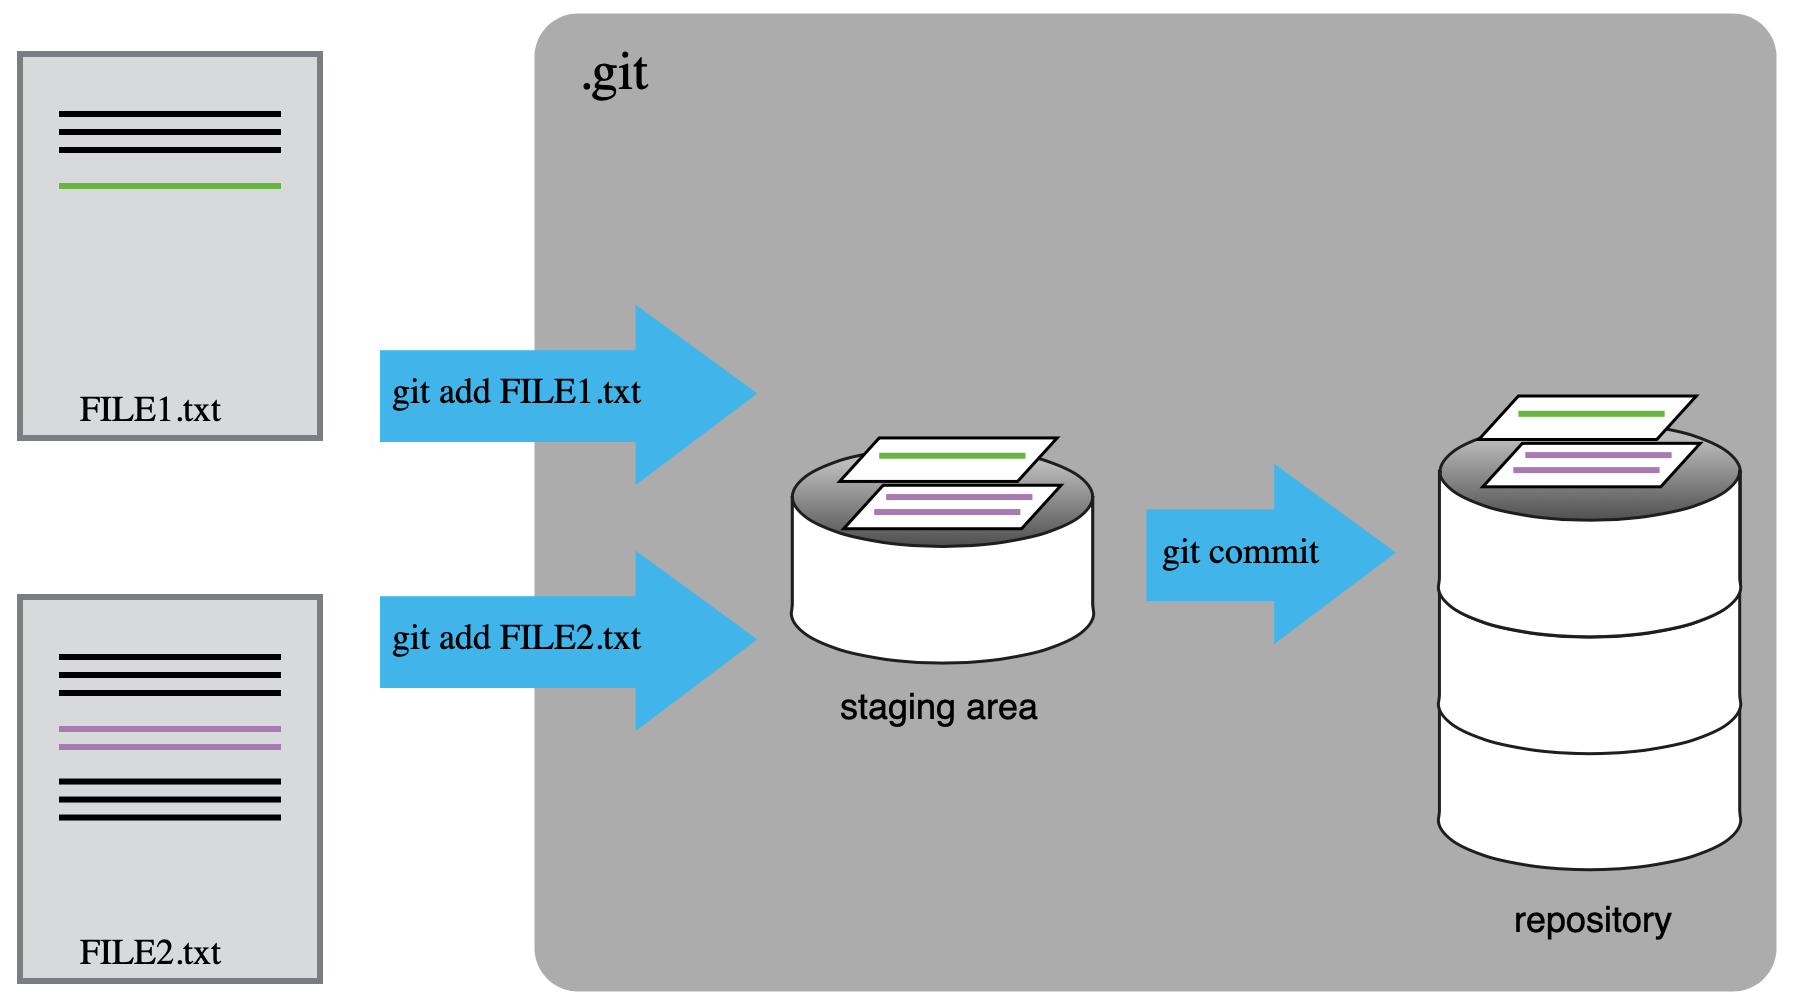
\includegraphics[width=0.95\textwidth]{sec2/git-committing.png}
  \end{figure}

\end{frame}

\begin{frame}[fragile]
\emptyframetitle

  Check the status
  \begin{lstlisting}[language=bash]
  $ git status
  \end{lstlisting}

  \begin{block}{Output if working directory / repository is brand new}
    \begin{lstlisting}[language=bash]
      On branch master
      No commits yet
      nothing to commit (create/copy files and use "git add" to track)
    \end{lstlisting}
  \end{block}

  \vspace{0.5cm}
  Now create a new file \texttt{hello\_world.py} in your working directory that prints 'Hello World!'

\end{frame}

\begin{frame}[fragile]
\emptyframetitle
  When you check the status again, you will now see there is an untracked file.
  \begin{lstlisting}[language=bash]
  $ git status
  \end{lstlisting}

  \begin{block}{Output if working directory differs, but new file is not yet being tracked}
    \begin{lstlisting}[language=bash]
      On branch master
      No commits yet
      Untracked files:
        (use "git add <file>..." to include in what will be committed)
              hello_world.py

      nothing added to commit but untracked files present (use "git add" to track)
    \end{lstlisting}
  \end{block}

\end{frame}


\begin{frame}[fragile]
\emptyframetitle
  Add your new file and start the tracking.
  \begin{lstlisting}[language=bash]
  $ git add hello_world.py
  \end{lstlisting}
  Check the status again  
  \begin{lstlisting}[language=bash]
  $ git status
  \end{lstlisting}
 
  \begin{block}{Output if working directory differs and file is being tracked}
    \begin{lstlisting}[language=bash]
      On branch master
      No commits yet
      Changes to be committed:
        (use "git rm --cached <file>..." to unstage)
              new file:   hello_world.py
    \end{lstlisting}
  \end{block}
\end{frame}

\begin{frame}[fragile]
\emptyframetitle

  Now commit the change and record it permanently.
  \begin{lstlisting}[language=bash]
  $ git commit -m 'Added new file'
  \end{lstlisting}

  \begin{block}{Output of \texttt{git commit}}
    \begin{lstlisting}[language=bash]
      [master (root-commit) b3557d4] Added new file
       1 file changed, 8 insertions(+)
       create mode 100644 hello_world.py
    \end{lstlisting}
  \end{block}
\end{frame}

\begin{frame}[fragile]
\emptyframetitle

  Check the status with \texttt{\textbf{git status}} and you get the following message:

  \begin{block}{}
    \begin{lstlisting}[language=bash]
      On branch master
      nothing to commit, working tree clean
    \end{lstlisting}
  \end{block}

  You can check the log to see your commits. The most recent appears first.

    \begin{lstlisting}[language=bash]
      $ git log
    \end{lstlisting}

  \begin{block}{}
    \begin{lstlisting}[language=bash]
      commit 249156049502e47d839735c34e31830885bc5092 (HEAD -> master)
      Author: Oliver Henrich <ohenrich@users.noreply.github.com>
      Date:   Wed Sep 2 16:56:07 2020 +0100
          Added new file
      \end{lstlisting}
  \end{block}
 
\end{frame}

\subsection{Exploring History}\hypertarget{sec2.4}{}

\begin{frame}[fragile]
\emptyframetitle

  When working with repos, you often want to \textbf{review changes before committing them} or \textbf{revert to a previous version} of the file.\\[0.25cm]

  Add an additional line to the previous \texttt{hello\_world.py} file. Check the \textbf{differences between your local and remote repository} with

  \begin{lstlisting}[language=bash]
    $ git diff
  \end{lstlisting}

  \begin{block}{Additional line \texttt{'print(`Hello Scotland!')'} in local file (+)}
    \begin{lstlisting}[language=bash]
      diff --git a/hello_world.py b/hello_world.py
      index 73fb7c3..e6f9107 100644
      --- a/hello_world.py
      +++ b/hello_world.py
      @@ -1 +1,2 @@
       print('Hello World!')
      +print('Hello Scotland!')
    \end{lstlisting}
  \end{block}

\end{frame}

\begin{frame}[fragile]
\emptyframetitle

  Commit the change 

  \begin{lstlisting}[language=bash]
    $ git add hello_world.py
    $ git commit -m 'Added additional line'
  \end{lstlisting}

  and check the differences again.

  \begin{lstlisting}[language=bash]
    $ git diff
  \end{lstlisting}

  There are no differences anymore as you committed your change.\\[0.25cm]

  Now check the status again.

  \begin{lstlisting}[language=bash]
    $ git status
  \end{lstlisting}
  \vspace*{-0.25cm}
  \begin{block}{Output of \texttt{git status}}
    \begin{lstlisting}[language=bash]
      On branch master
      nothing to commit, working tree clean
    \end{lstlisting}
  \end{block}

\end{frame}

\begin{frame}[fragile]
\emptyframetitle

  Add another line, commit the change again and check your commit log.

  \begin{columns}
    \begin{column}{0.55\textwidth}
      \begin{block}{Output of \texttt{git log}}
        \begin{lstlisting}[language=bash, basicstyle=\tiny\ttfamily]
          commit 908944eb711c90f5bd46297639b34d8fc70993f0 (HEAD -> master)
          Author: Oliver Henrich <ohenrich@users.noreply.github.com>
          Date:   Wed Sep 2 16:59:00 2020 +0100
              Added another additional line

          commit 28f46c36b5729ab26ca719cc1468b1a6e734d597
          Author: Oliver Henrich <ohenrich@users.noreply.github.com>
          Date:   Wed Sep 2 16:58:15 2020 +0100
              Added additional line

          commit 249156049502e47d839735c34e31830885bc5092
          Author: Oliver Henrich <ohenrich@users.noreply.github.com>
          Date:   Wed Sep 2 16:56:07 2020 +0100
              Added new file
        \end{lstlisting}
      \end{block}
    \end{column}

    \begin{column}{0.425\textwidth}
      \vspace*{0.cm}\\
      \textbf{All commits have a unique ID}, but Git knows a simple way to address them:\\
      \vspace*{0.4cm}
      The \textbf{last commit} appears at the top and is marked with \texttt{\textbf{HEAD}}.
      \vspace*{0.7cm}\\
      The \textbf{two previous commits} are not marked, but can be conveniently addressed with \textbf{\texttt{HEAD\textasciitilde1}} and \textbf{\texttt{HEAD\textasciitilde2}}.
    \end{column}
  \end{columns}

\end{frame}

\begin{frame}[fragile]
\emptyframetitle

  If we want to see what the differences are between the current version (\texttt{\textbf{HEAD}}) and version two commits ago, we can issue for instance

  \begin{lstlisting}[language=bash]
    $ git diff HEAD~2
  \end{lstlisting}

  \begin{block}{Additional two lines marked as different in local file (+)}
    \begin{lstlisting}[language=bash]
      diff --git a/hello_world.py b/hello_world.py
      index 73fb7c3..547a19b 100644
      --- a/hello_world.py
      +++ b/hello_world.py
      @@ -1 +1,3 @@
       print('Hello World!')
      +print('Hello Scotland!')
      +print('Hello Glasgow!')
    \end{lstlisting}
  \end{block}
\end{frame}

\begin{frame}[fragile]
\emptyframetitle

  Assume you want to obtain the previous version without the additional line.\\[0.2cm]

  First you need to \textbf{check the log for the ID of the previous commit}.

  \vspace*{-0.2cm}
  \begin{columns}
      \begin{column}{0.55\textwidth}
        \begin{block}{Output of \texttt{git log}}
          \begin{lstlisting}[language=bash, basicstyle=\tiny\ttfamily]
            commit 28f46c36b5729ab26ca719cc1468b1a6e734d597
            Author: Oliver Henrich <ohenrich@users.noreply.github.com>
            Date:   Wed Sep 2 16:58:15 2020 +0100
                Added additional line
          \end{lstlisting}
        \end{block}
      \end{column}
      \begin{column}{0.425\textwidth}
        \vspace*{0.5cm}\\
        The commit ID is the long bit starting 28f46c36b5\dots\\[0.25cm]
         It is \textbf{usually sufficient to specify only 7 digits}.
      \end{column}
    \end{columns}

  \vspace*{0.2cm}
  Use the \texttt{\textbf{git checkout}} command to retrieve a previous version.

  \begin{lstlisting}[language=bash]
    $ git checkout 28f46c36b5 hello_world.py
  \end{lstlisting}

  \textcolor{red}{\textbf{Note: Do not forget the filename at the end as this will 'detach the \texttt{HEAD}'}!}\\[0.2cm]

  To \textbf{retrieve the latest version} again use 

  \begin{lstlisting}[language=bash]
    $ git checkout master hello_world.py
  \end{lstlisting}


\end{frame}

\begin{frame}[fragile]
\emptyframetitle
  The previous command will not revert the commit (check e.g. \texttt{\textbf{git log}}).\\[0.25cm]

  To \textbf{revert an erroneous commit, first look for its ID} and use \texttt{\textbf{git revert}}.

  \begin{columns}
    \begin{column}{0.55\textwidth}
      \begin{block}{Output of \texttt{git log}}
        \begin{lstlisting}[language=bash, basicstyle=\tiny\ttfamily]
          commit 908944eb711c90f5bd46297639b34d8fc70993f0 (HEAD -> master)
          Author: Oliver Henrich <ohenrich@users.noreply.github.com>
          Date:   Wed Sep 2 16:59:00 2020 +0100
              Added another additional line

          commit 28f46c36b5729ab26ca719cc1468b1a6e734d597
          Author: Oliver Henrich <ohenrich@users.noreply.github.com>
          Date:   Wed Sep 2 16:58:15 2020 +0100
              Added additional line
        \end{lstlisting}
      \end{block}
    \end{column}

    \begin{column}{0.425\textwidth}
      \vspace*{1.cm}\\
      We want to revert the commit starting 908944eb71\dots
      \vspace*{0.8cm}\\
      We want the current version to be this one.
    \end{column}
  \end{columns}


  \begin{lstlisting}[language=bash]
    $ git revert 908944eb71 
  \end{lstlisting}

  This creates a new commit with the previous version of the file.

\end{frame}

\begin{frame}[fragile]
\emptyframetitle

\vspace*{-0.75cm}
  \begin{columns}
    \begin{column}{0.55\textwidth}
      \begin{figure}[h]
        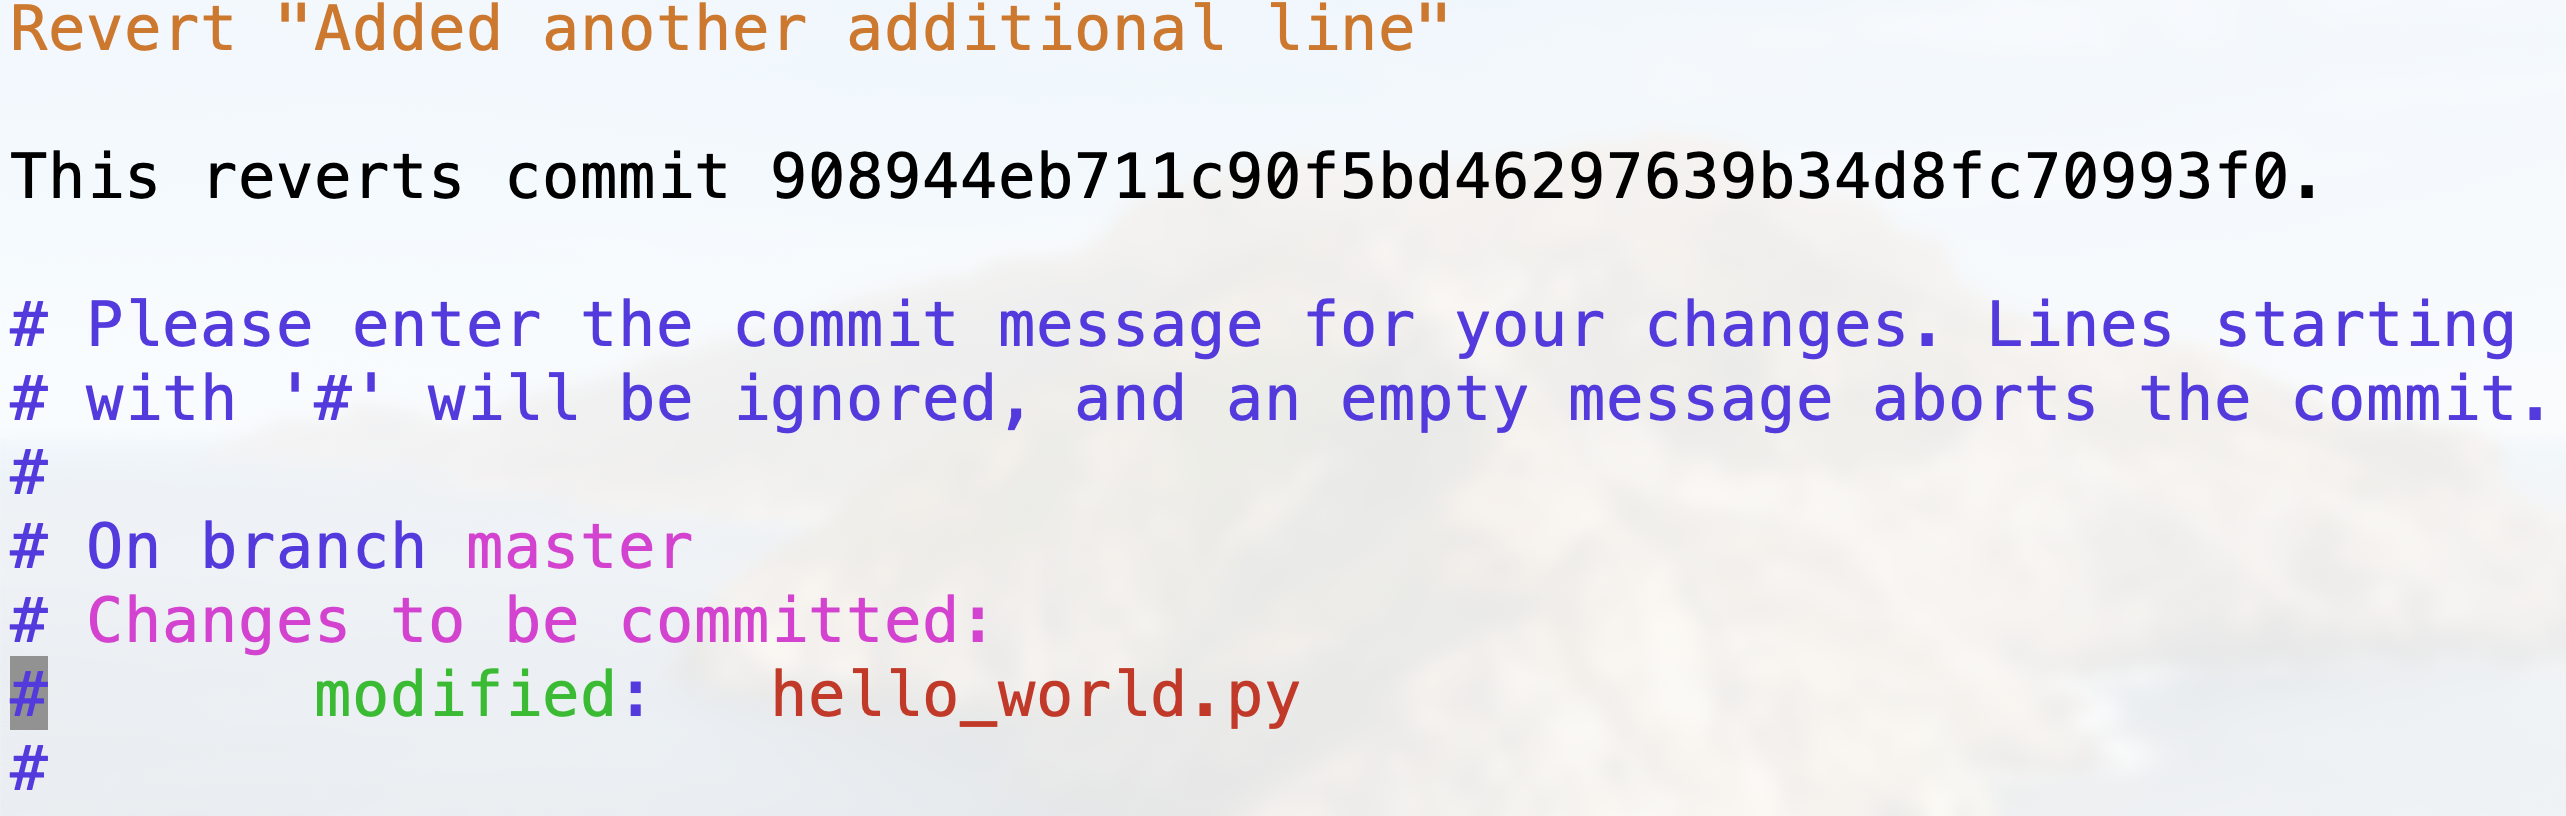
\includegraphics[width=1.0\textwidth]{sec2/git-revert.png}
      \end{figure}

    \end{column}

   \begin{column}{0.45\textwidth}
      \vspace*{0.5cm}\\
      A dialogue window opens that asks you for a message providing a template.
    \end{column}
  \end{columns}

\vspace*{-0.2cm}
  \begin{columns}
    \begin{column}{0.7\textwidth}

      \begin{block}{}
        \begin{lstlisting}[language=bash, basicstyle=\tiny\ttfamily]
          commit 15f36c3bd31f594504756326df6b3baeb2d0982c (HEAD -> master)
          Author: Oliver Henrich <ohenrich@users.noreply.github.com>
          Date:   Thu Sep 3 17:29:03 2020 +0100
              Revert "Added another additional line"
              This reverts commit 908944eb711c90f5bd46297639b34d8fc70993f0.

          commit 908944eb711c90f5bd46297639b34d8fc70993f0
          Author: Oliver Henrich <ohenrich@users.noreply.github.com>
          Date:   Wed Sep 2 16:59:00 2020 +0100
              Added another additional line

          commit 28f46c36b5729ab26ca719cc1468b1a6e734d597
          Author: Oliver Henrich <ohenrich@users.noreply.github.com>
          Date:   Wed Sep 2 16:58:15 2020 +0100
              Added additional line

          commit 249156049502e47d839735c34e31830885bc5092
          Author: Oliver Henrich <ohenrich@users.noreply.github.com>
          Date:   Wed Sep 2 16:56:07 2020 +0100
              Added new file
        \end{lstlisting}
      \end{block}
    \end{column}

     \begin{column}{0.25\textwidth}
        \vspace*{0.5cm}\\
        Your commit log has now an extra entry.
    \end{column}
  \end{columns}


\end{frame}


